\section{Evaluation}

Our tests were ran on the QEMU Linux emulator, with a VM simulating a machine with some stuff. We ran our tests on several main memory sizes, as the Linux cache will use as much as it can before the memory needs to be used by another process, and we wanted to force eviction as much as possible, since it is the core of our modified policy. We evaluate our implementation against the default Linux page caching implementation using a few benchmarks:

\begin{itemize}
	\item Cscope benchmark: 
	\item Postgres benchmark:
\end{itemize}


\label{fig:cscope}
\begin{figure}[h]
	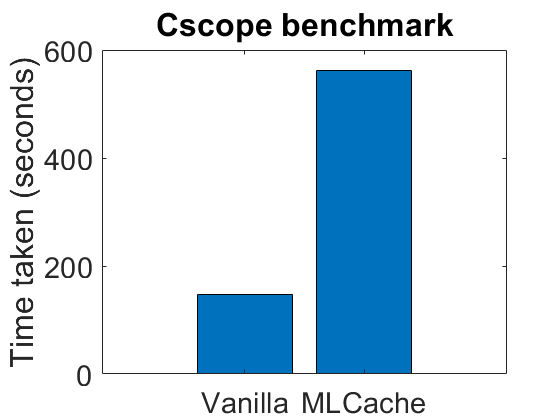
\includegraphics[scale=0.4]{img/cscope_results_bigger.png}
	\caption{Cscope benchmark results for the unmodified Linux kernel versus our MLCache prototype, ran on a VM with 256MB RAM.}
\end{figure}


The results from the Cscope benchmark give us some sense of the overhead caused by our implementation, as the current Linux implementation does not benefit very much from caching for this benchmark. We can see that the time taken was about 3x on MLCache. This is not surprising, as we have to update each page's scores in the cache on every reference, as well as doing a linear scan over Linux's linked list on eviction. Thus, the current overhead for score maintenance is quite large.

\label{fig:pg}


\begin{figure}[h]
	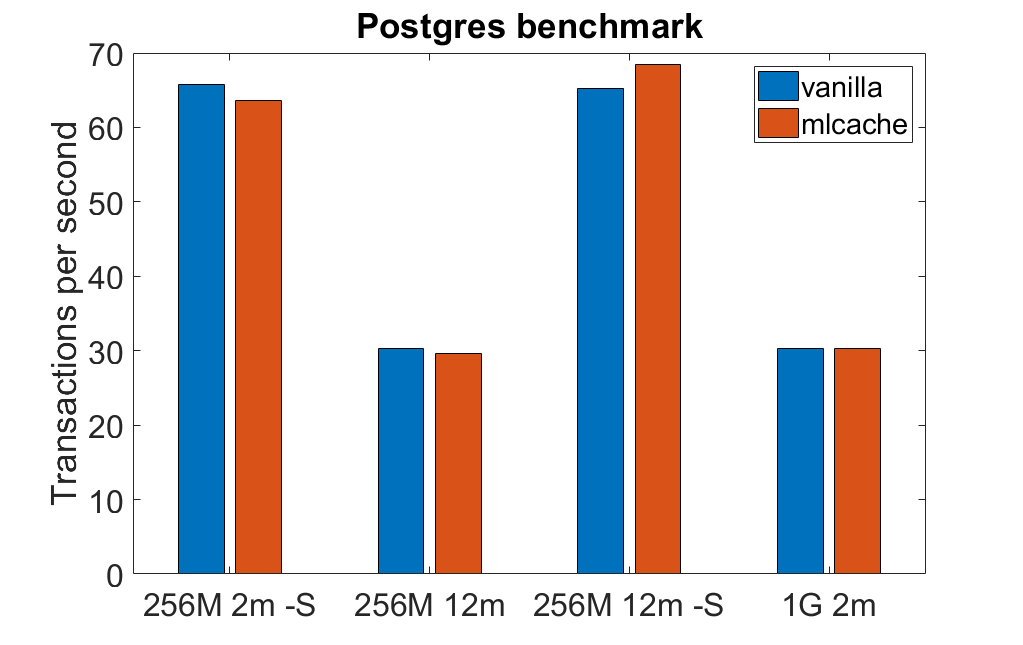
\includegraphics[scale=0.3]{img/postgres_results_bigger.png}
	\caption{Postgres benchmark results for the unmodified Linux kernel versus our MLCache prototype, with different RAM sizes. The -S command means just reads, no writes.}
\end{figure}

Our results from the Postgres benchmark show us that even with the extra machinery we have built on top of Linux, we achieve similar performance, especially as memory decreases and on longer runs. This is probably due to the current implementation having to develop new scores from scratch on every run, and so reaching accurate scores takes some time. After 12 minutes, however, our design starts to outperform Linux. This is relatively fast, since training would ideally be done only once, and the rest is online learning. We should note that our implementation takes advantage of smaller memory sizes due to the increased amount of evictions done: without any evictions, our design is pure overhead.

As a small experiment, we also tested how our implementation fared when evicting the lowest score (best) pages every time. For the Cscope benchmark, it took about 3 hours to complete. This gives us some proof that our algorithm, although not ideal, is in the right direction, compared to a completely naive implementation. 

Our implementation also introduces a small memory overhead on the Linux page struct. We add two longs to keep track of the scores and the number of times a page has been evicted. This causes an increase of 15\% memory usage for each page on the x86 architecture.